\newif\ifvimbug
\vimbugfalse

\ifvimbug
\begin{document}
\fi


\subsection{Marching Cubes (3 Punkte)}
\subsubsection{1 Punkt}
Alle blauen Punkte sind innen, alle grünen außen. Die roten Linien sind die eindeutigen Kanten / Zellen und die Zellen mit den orangenen und gelben Linien sind uneindeutig. Hierbei kann entweder orange oder gelb gewählt werden. \\
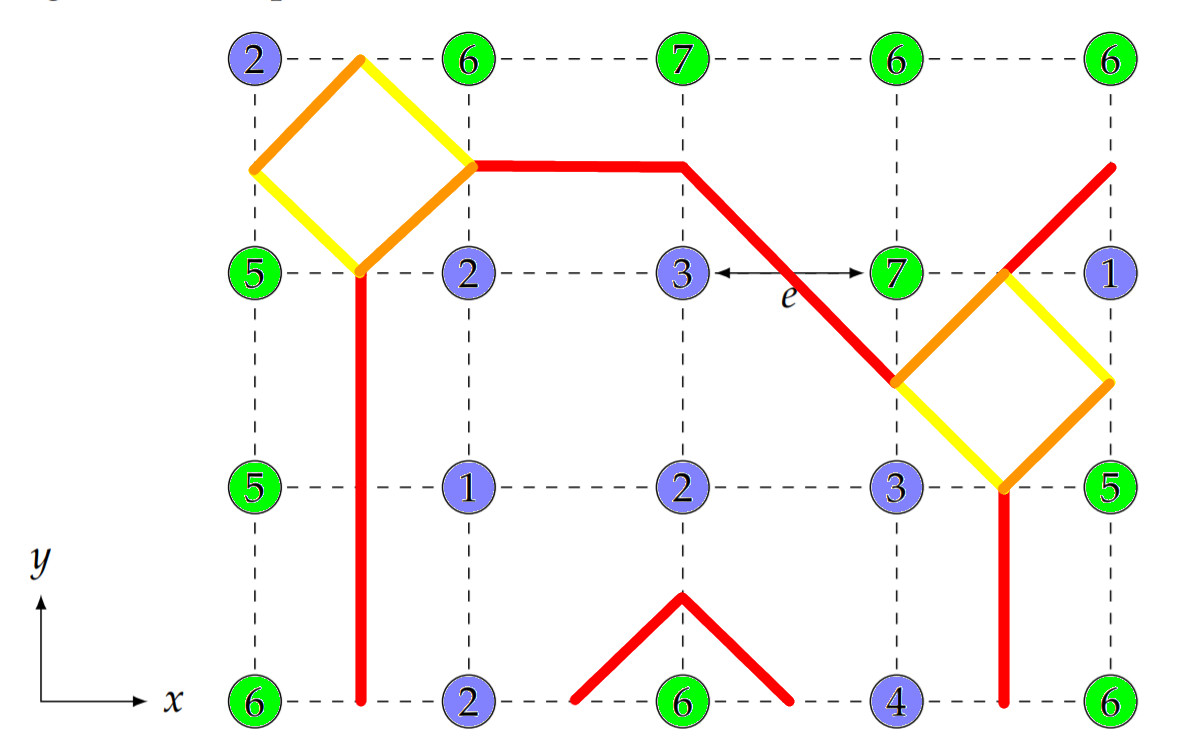
\includegraphics[width=(\textwidth/2)]{51a.jpg} 
\subsubsection{1 Punkt}
\subsubsection{1 Punkt}